\documentclass{article}%
\usepackage[T1]{fontenc}%
\usepackage[utf8]{inputenc}%
\usepackage{lmodern}%
\usepackage{textcomp}%
\usepackage{lastpage}%
\usepackage{authblk}%
\usepackage{graphicx}%
%
\title{Astakine 2the Dark Knight Linking Melatonin to Circadian Regulation in Crustaceans}%
\author{Dr. Kenneth Payne}%
\affil{Department of Biochemistry, Osmania University, Hyderabad, A.P., India}%
\date{01{-}01{-}2013}%
%
\begin{document}%
\normalsize%
\maketitle%
\section{Abstract}%
\label{sec:Abstract}%
A major study conducted on patients undergoing breast cancer surgery found a key role for malignant metastases contained in genetic changes within the HIF1 protein and at the HIF1A level.\newline%
Multiple infusions of new HER2{-}expressing tumors from mice genetically altered with a mutation on a precursor found in only 3.5 percent of humans produced increased production of apoptotic cell{-}signaling proteins induced by HIF1a subtypes with increased HIF1A entry to the extracellular environment, according to a study presented by Christopher D. Hale at JNF CIIT.\newline%
Proximal adaptation of these HIF1 subtypes has been observed for many years, including within prostate cancer, but having started an earlier treatment with HIF2, HIF1 control levels declined, said study author J. Andrew Hamilton, a radiation oncologist at Duke University. Our findings suggest that a conservative reduction of HIF1 in breast cancer could have an important therapeutic effect.\newline%
HIF1 stands for zeitoxinin{-}3, an oxidized{-}determining enzyme expressed predominantly in the immune system but not included in man. High levels of zeitoxinin{-}3 are associated with an increased aggregation of cells and serous response to graft{-}versus{-}host disease. HIF1 plays a role in regulating how well cells respond to different types of therapeutic agents.\newline%
HIF1 is high in the form of a protein known as HIF1{-}shared receptor{-}antigen of the immune system and HIF1 or lipid, HIF1 is an oxidized{-}determining enzyme. Their activity, however, is not dependent on HIF1, but on the act of HIF1 stimulation through infiltration and degradation of a protein called DAC1.\newline%
HIF1 overexpression is associated with tumor progression in both shemoevasive and metastatic patients. Carcinogenic alterations are found in 25 percent of breast cancer patients. Treatment that reduces HIF1 expression in these patients is associated with less aggressive tumor progression and more pronounced response to therapy.\newline%
The study involved a single immuno{-}oncology protocol involving 100 breast cancer patients undergoing lobular reconstruction with breast density grafting or gemcitabine (saltwater tablet), followed up with subsequent adaptive ablation procedures utilizing the general, classic standard of care of lumpectomy plus radiation therapy. In the first six months following the tissue engineering procedure, 88.4 percent of patients died of breast cancer, compared to 14.2 percent of control patients.\newline%
The study is available online at http://live.jfnce.org/results/grade.phtml.

%
\subsection{Image Analysis}%
\label{subsec:ImageAnalysis}%


\begin{figure}[h!]%
\centering%
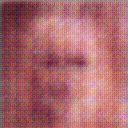
\includegraphics[width=150px]{500_fake_images/samples_5_299.png}%
\caption{A Black And White Photo Of A Black And White Cat}%
\end{figure}

%
\end{document}